\chapter{Bezpieczeństwo komunikacji}
\label{ch:communication security}

Jednym z podstawowych wymagań tej pracy jest bezpieczna wymiana komunikatów poprzez Bluetooth Low Energy. Za pomocą tego protokołu, poprzez bezprzewodowe medium, przesyłane są kluczowe dane, zwłaszcza komendy deaktywujące tryb alarmowy urządzenia. Transmisja jest zawsze realizowana rozgłoszeniowo, co powoduje, że jej podsłuchanie nie jest trudnym zadaniem. Jest to niebezpieczne z dwóch powodów. Pierwszym z nich jest fakt wysyłania wrażliwych danych, jak na przykład danych lokalizujących pojazd. Dzięki nim, potencjalny złodziej mógłby po krótkiej analizie bezproblemowo określić miejsca, w których regularnie przebywa pojazd, a następnie wybrać dla niego najbardziej korzystne i przygotować się do kradzieży. Po drugie, będąc w pobliżu pojazdu w trakcie wyłączania trybu alarmowego, byłby w stanie podsłuchać komendę deaktywującą, a następnie zapisać ją w celu późniejszego odtworzenia, co umożliwiłoby kradzież pojazdu.

Z przytoczonych powyżej powodów, komunikacja bezprzewodowa musi być szyfrowana. Jednakże operacja ta sama w sobie nie zabezpiecza komendy deaktywującej, a jedynie wrażliwe dane. Wynika to z faktu, iż w przypadku przechwycenia danych przesyłanych bezprzewodowo, dzięki szyfrowaniu są one nadal bezpieczne, ponieważ zmienny charakter. Inaczej jest w przypadku stałej komendy autoryzującej. Wynika to z faktu, że nie musi być ona tak naprawdę deszyfrowana przez potencjalnego złodzieja. Wystarczy, że jedynie ją odtworzy, nawet w formie zaszyfrowanej. Urządzenie wówczas ją zdeszyfruje i wykona deaktywację alarmu. W wyniku szyfrowania stałej komendy stałym kluczem szyfrującym, uzyskamy oczywiście również stały i powtarzalny pakiet zaszyfrowanych danych, które mogą być bezcenne w ręku potencjalnego złodzieja. W celu zabezpieczenia się przed tym, do komunikacji należy wprowadzić element zmienności w czasie.  

\section{AES}

Jako główny algorytm szyfrowania w niniejszej pracy wykorzystano algorytm AES (ang. Advanced Encryption Standard) w wersji ze 128-bitowym kluczem szyfrującym.  Wyboru tego dokonano, ponieważ zastosowany w pracy mikrokontroler nRF52832 firmy Nordic Semiconductor posiada sprzetowe wsparcie szyfrowania danych wykorzystując właśnie AES128. Algorytm ten powstał w 2001 roku w Stanach Zjednoczonych w ośrodku NIST (ang. National Institude of Standards and Technology) w wyniku prac badawczych dwóch belgijskich kryptografów - Vincenta Rijmena i Joan’a Daemen, od których nazwisk powstała oryginalna nazwa algorytmu – Rijndael. Stanowi on jeden z najpopularniejszych na świecie szyfrów symetrycznych, a o jego skuteczności stanowi fakt, że w 2002r. został przyjęty jako federalny standard szyfrowania w Stanach Zjednoczonych. Pojęcie szyfr symetryczny oznacza, że do zaszyfrowania oraz zdeszyfrowania stosuje się ten sam klucz szyfrujący (w przeciwieństwie do algorytmów asymetrycznych, gdzie stosuje się dwa klucze, jeden do szyfrowania, a drugi do deszyfracji). Z tego powodu, klucz szyfrujący stanowi ekstremalnie wrażliwe dane, które pod żadnym pozorem nie powinno się przesyłać poprzez ogólno dostępne medium komunikacyjne. Wyciek klucza szyfrującego powoduje zagrożenie bezpieczeństwa komunikacji.
Proces szyfrowania składa się z kilku kroków. Pierwszym z nich jest podzielenie danych wejściowych (zwyczajowo nazywanych tekstem jawnym) na bloki o rozmiarze 128 bitów, czyli szesnastu bajtów. Każdy blok przedstawiany jest jako macierz o wymiarach 4 bajty x 4 bajty, szeregowana kolumnami. Macierze te nazywają się macierzami stanu. Następnie, na każdej z tych macierzy (bloku danych) wykonywane są kolejne operacje:

\begin{enumerate}
\item  Utworzenie podkluczy – etap ten polega na wygenerowaniu w sposób losowy klucza pierwotnego, a następnie na jego podstawie - po jednym podkluczu dla każdej z rund szyfrujących. Ich liczba jest uzależniona od rozmiaru klucza. Dla klucza 128-bitowego występuje 10 rund, dla klucza 192-bitowego – 12, a dla klucza 256-bitowego – 14 powtórzeń, wliczając klucz pierwotny.

\item Wykonanie rundy wstępnej (inicjującej). Polega na wykonaniu operacji alternatywy wyłączanej – XOR (\textit{ang. Exclusive Or}) dla każdego bajtu z bloku danych oraz odpowiadającego mu bajtu w kluczu pierwotnym.

\item Wykonanie rund szyfrujących – Etap ten jest wykonywany kilkukrotnie, w zależności od liczby cykli. Każda runda składa się z kilku kroków. 

	\begin{itemize}
	\item W pierwszym z nich, każdy bajt danych jest zastępowany innym bajtem pobranym ze zdefiniowanej tablicy (\textit{ang. lookup table}) nazywanej S-Boxe’em Rijndael’a. Operacja ta nazywa się w skrócie SB (\textit{ang. \textbf{S}ubstitude \textbf{B}ytes}) i przedstawiono ją na rysunku \ref{fig:image_substitute_bytes}. Zgodnie z zamysłem twórców, tablica ta gwarantuje nieliniowość przekształcenia, a w efekcie i całego szyfrowania.
	
	\begin{figure}[h]
		\centering
		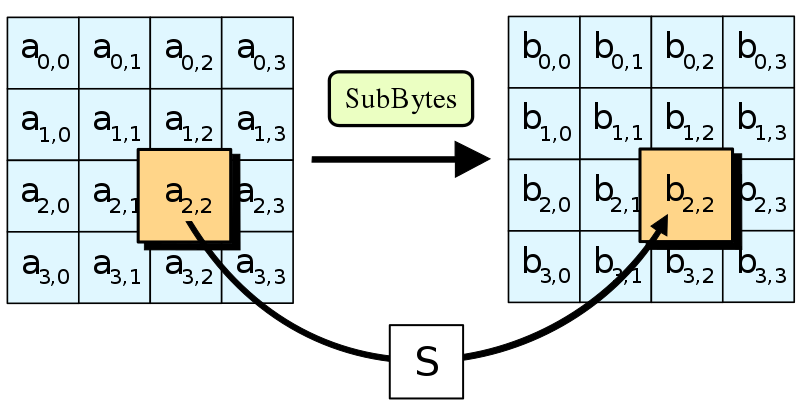
\includegraphics[width=10cm]{img/com_security/800px-AES-SubBytes.png}
		\caption{Wykonanie operacji Substitute Bytes. Źródło: \cite{aes_wiki}.}
		\label{fig:image_substitute_bytes}
	\end{figure}

	\item  Kolejny krok to zamiana wierszy. Polega na przesunięciu bajtów w trzech ostatnich wierszach bloku. Pierwszy wiersz pozostaje bez zmian, w drugim wierszu bajty są przesuwane o jeden w lewo, w trzecim o dwie pozycje w lewo, a w ostatnim o 3 miejsca w tym samym kierunku. Każdy bajt, który w wyniku przesunięcia znajdzie się poza wierszem, zostaje umieszczony na jego ostatniej pozycji (wiersze w wyniku rotacji się zawijają). Operacja ta nosi miano SR (\textit{ang. \textbf{S}hift \textbf{R}ows}). Przedstawiono ją na rysunku \ref{fig:image_shift_rows}.
	
	\begin{figure}[h]
		\centering
		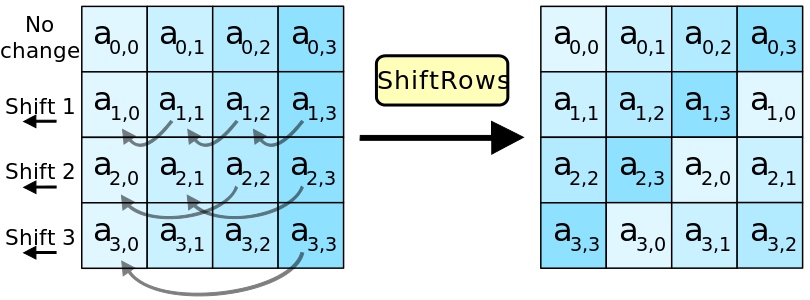
\includegraphics[width=10cm]{img/com_security/810px-AES-ShiftRows.png}
		\caption{Wykonanie operacji Shift Rows. Źródło: \cite{aes_wiki}.}
		\label{fig:image_shift_rows}
	\end{figure}
	
	\item Trzecim z kolei krokiem jest operacja mieszania kolumn – MC (\textit{ang. \textbf{M}ix \textbf{C}olumns}). W tym etapie, każda z kolumn jest przemnażana lewostronnie przez stałą macierz o wymiarach 4 x 4, w wyniku czego powstaje kolumna z nowymi wartościami. Operacja ta przedstawiona jest na rysunku \ref{fig:image_mix_columns}.
	
	\begin{figure}[H]
		\centering
		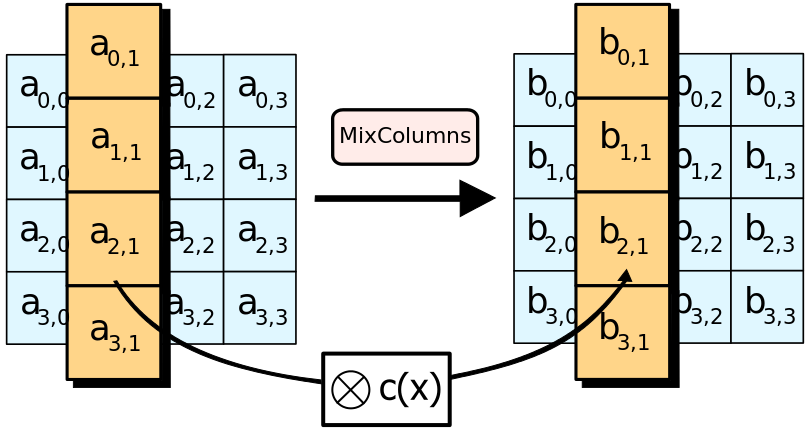
\includegraphics[width=10cm]{img/com_security/810px-AES-MixColumns.png}
		\caption{Wykonanie operacji Mix Columns. Źródło: \cite{aes_wiki}.}
		\label{fig:image_mix_columns}
	\end{figure}
	
	\item Ostatni krok nazywany jest AR (\textit{ang. \textbf{A}dd \textbf{R}ound Key}) i polega na wykonaniu operacji XOR na każdym bajcie bloku danych i odpowiadającym mu bajcie w kluczu przypisanym do danej rundy. Wizualizację kroku przedstawiono na rysunku \ref{fig:image_round_keys}.
	
	\begin{figure}[h]
		\centering
		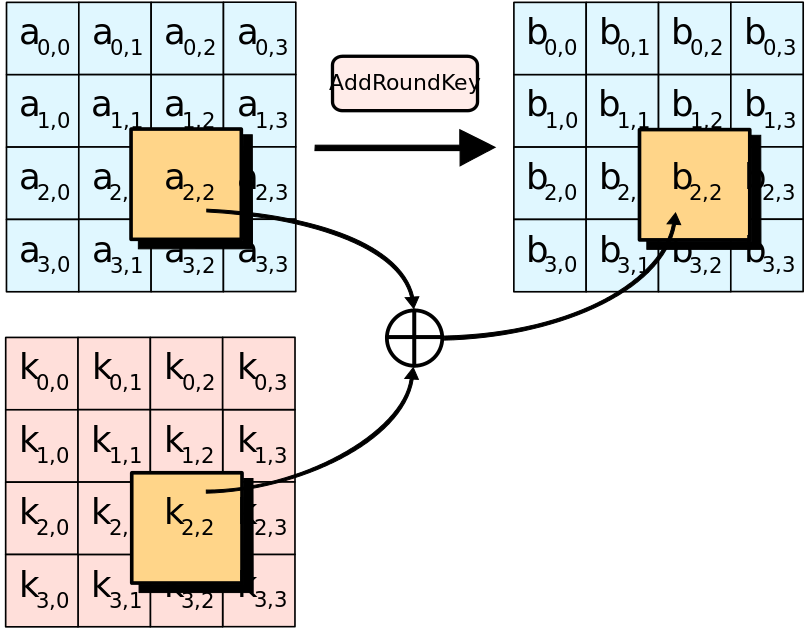
\includegraphics[width=10cm]{img/com_security/810px-AES-AddRoundKey.png}
		\caption{Wykonanie operacji Add Round Key. Źródło: \cite{aes_wiki}.}
		\label{fig:image_round_keys}
	\end{figure}
	\end{itemize}
	
\item Ostatni etap to runda kończąca – W jej trakcie wykonywane są operacje identyczne jak w rundach szyfrujących, za wyłączeniem mnożenia kolumn, które nie występuje.

\end{enumerate}

Deszyfrowanie jest operacją odwrotną do szyfrowania i polega na przekształceniu danych zaszyfrowanych na tekst jawny. Tak samo jak w przypadku szyfrowania, tekst dzieli się na 16-bajtowe bloki. W jego trakcie wykonuje się analogiczne operacje co w przypadku szyfrowania.

\begin{enumerate}
\item Odwrotne podstawianie bajtów – polega na ponownym zastosowaniu tablicy S-Box w celu podmiany bajtów.

\item Przesuwanie bajtów w wierszach w prawo. Zasada jest taka sama jak w operacji SR, zmienia się jedynie kierunek.

\item Wykonanie operacji XOR dla każdego bajtu bloku danych z odpowiadającym mu bajtem w podkluczu przypisanym do danej rundy deszyfrującej. Podklucze są takie same jak w trakcie szyfrowania, lecz powinny być brane w kolejności odwrotnej (zaczynając od ostatniego, a kończąc na kluczu pierwotnym).

\item Ostatnia operacja to odwrócone mnożenie kolumn.

\end{enumerate}

W efekcie uzyskujemy blok danych zdeszyfrowanych.
Przedstawiony tutaj wariant algorytmu szyfrowania nosi miano ECB (\textit{ang. \textbf{E}lectronic \textbf{C}ode\textbf{b}ook}) i stanowi najprostszą metodę szyfrowania. Można go przedstawić na rysunkach \ref{fig:image_ecb_encrypt} oraz \ref{fig:image_ecb_decrypt}.

	\begin{figure}[h]
		\centering
		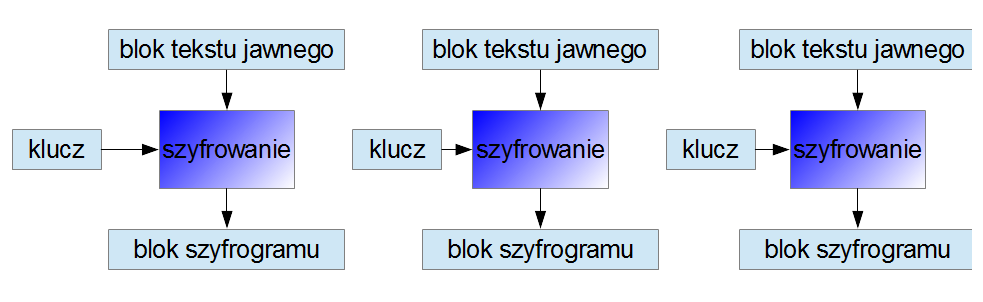
\includegraphics[width=15cm]{img/com_security/ECB_szyfrowanie.png}
		\caption{Operacja szyfrowania metodą ECB. Źródło: \cite{aes_cryptoit}.}
		\label{fig:image_ecb_encrypt}
	\end{figure}
	
	\begin{figure}[h]
		\centering
		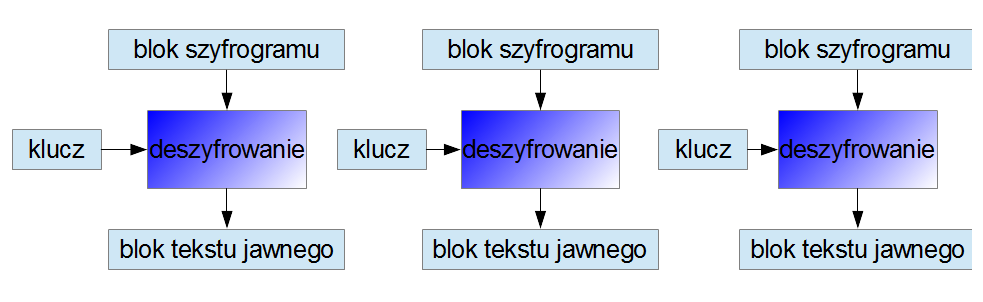
\includegraphics[width=15cm]{img/com_security/ECB_deszyfrowanie.png}
		\caption{Operacja deszyfrowania metodą ECB. Źródło: \cite{aes_cryptoit}.}
		\label{fig:image_ecb_decrypt}
	\end{figure}
	
Czas trwania szyfrowania pojedynczego bloku danych o długości szesnastu bajtów na mikrokontrolerze nRF52832 wynosi w przybliżeniu 30 $\mu s$. Deszyfrowanie trwa zaś około 60 $\mu s$.


\section{Dodatkowe warianty szyfrowania AES}

Jak zostało przedstawione wcześniej, mechanizmy szyfrowania doskonale działają w przypadku wrażliwych danych. Nie sprawdzają się natomiast w przypadku przesyłania komend, ze względu na brak zmienności pakietów w czasie i możliwości odtworzenia zaszyfrowanego pakietu przez niepowołane osoby. Z tego powodu, do komunikacji należy wprowadzić element zmienności.
Jednym z wariantów algorytmu AES jest tzw. CFB (\textit{ang. \textbf{C}ipher \textbf{F}eed\textbf{b}ack}), przedstawiony na rysunkach \ref{fig:image_cfb_encrypt} oraz \ref{fig:image_cfb_decrypt}. Stanowi on wysokopoziomowy algorytm, który bazuje na wariancie ECB, zmieniając jedynie logiczną strukturę informacji niezbędnych do szyfrowania. Przede wszystkim, wprowadza pojęcie wektora inicjującego (\textit{ang. initializing vector}), który stanowi niezbędny dodatkowy element zmienności. Klucz główny jest zazwyczaj niezmienny dla pary komunikujących się ze sobą urządzeń, co w rezultacie wprowadza konieczność nieupubliczniania go. Wektor inicjujący jest natomiast generowany przy każdej nowej komunikacji. 

	\begin{figure}[h]
		\centering
		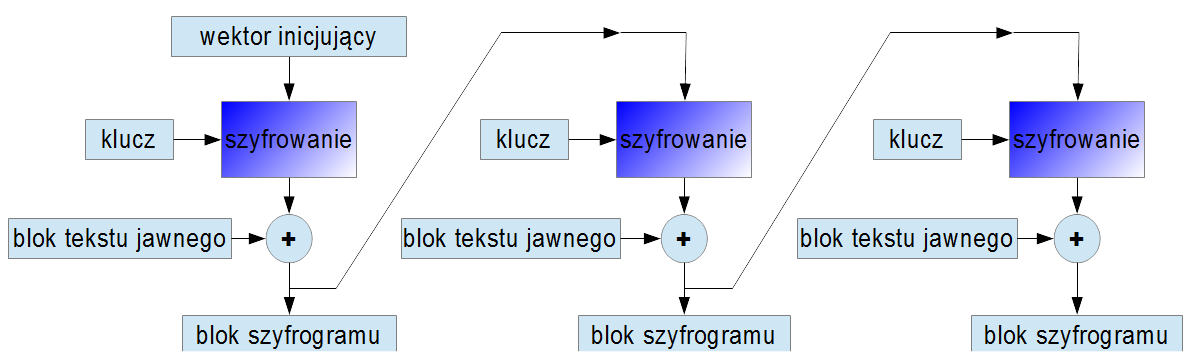
\includegraphics[width=15cm]{img/com_security/CFB_szyfrowanie.png}
		\caption{Operacja szyfrowania metodą CFB. Źródło: \cite{aes_cryptoit}.}
		\label{fig:image_cfb_encrypt}
	\end{figure}
	
	\begin{figure}[h]
		\centering
		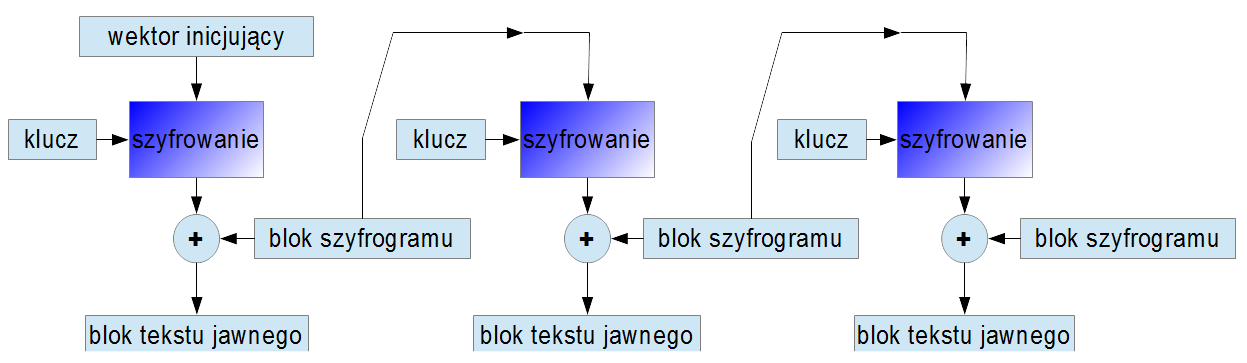
\includegraphics[width=15cm]{img/com_security/CFB_deszyfrowanie.png}
		\caption{Operacja deszyfrowania metodą CFB. Źródło: \cite{aes_cryptoit}.}
		\label{fig:image_cfb_decrypt}
	\end{figure}
	

W odróżnieniu od wariantu ECB, zamiast tekstu jawnego szyfrowaniu ulega wektor inicjujący. Jego postać zaszyfrowana jest następnie poddawana operacji XOR z blokiem danych tekstu jawnego, a powstały w ten sposób szyfrogram stanowi nowy wektor inicjujący dla następnego bloku danych.
W przypadku deszyfrowania korzysta się oczywiście z tego samego wektora inicjującego oraz klucza szyfrującego. Co ciekawe, w odróżnieniu od wariantu ECB, w metodzie CFB deszyfrowanie jest to tak naprawdę szyfrowanie. Oznacza to, że wystarczy zaimplementować jedynie mechanizm szyfrowania w algorytmie AES, aby móc zarówno szyfrować jak i deszyfrować wiadomości. Zaszyfrowany wektor inicjujący jest poddawany operacji XOR z blokiem tekstu zaszyfrowanego w efekcie czego uzyskujemy blok tekstu jawnego. Natomiast blok tekstu zaszyfrowanego stanowi wektor inicjujący dla następnych bloków szyfru.


\section{Realizacja szyfrowania komunikacji w projekcie}
W pracy zdecydowano się na wykorzystanie zarówno metod ECB oraz CFB. Pierwszym, a zarazem najbardziej podstawowym etapem jest generowanie klucza szyfrującego. Operacja ta jest realizowana przez płytę główną systemu lokalizującego. Następnie, klucz jest przekazywany w trakcie inicjalizacji porzez interfejs NFC (\textit{ang. \textbf{N}ear \textbf{F}ield \textbf{C}ommunication}) do urządzenia deaktywującego, pełniącego rolę beacona (urządzenia rozgłaszającego). Zastosowanie NFC jest powszechnie uważane za bezpieczną metodę komunikacji, ze względu na jej bardzo niską moc transmisji, a tym samym bardzo niewielki zasięg (do 10 cm). Ogranicza to zatem możliwość podsłuchania klucza szyfrującego do zera. Przy pomocy tego klucza, za każdym razem gdy płyta główna systemu połączy się z urządzeniem deaktywującym w celu uzyskania od niego komendy deaktywującej, wpierw wysłany zostanie zaszyfrowany, nowo wygenerowany na potrzeby danego połączenia wektor inicjalizacyjny. Umożliwi to dalszą komunikację wykorzystując wariant CFB oraz niezbędną zmienność zaszyfrowanych pakietów, praktycznie niwelującą skuteczność podsłuchiwania transmisji. 